\section{Implementazione}
In questo capitolo bla bla bla

\subsection{Strumenti}
- abbiamo usato matlab
- codice è su github


\begin{figure}[ht]
\begin{center}
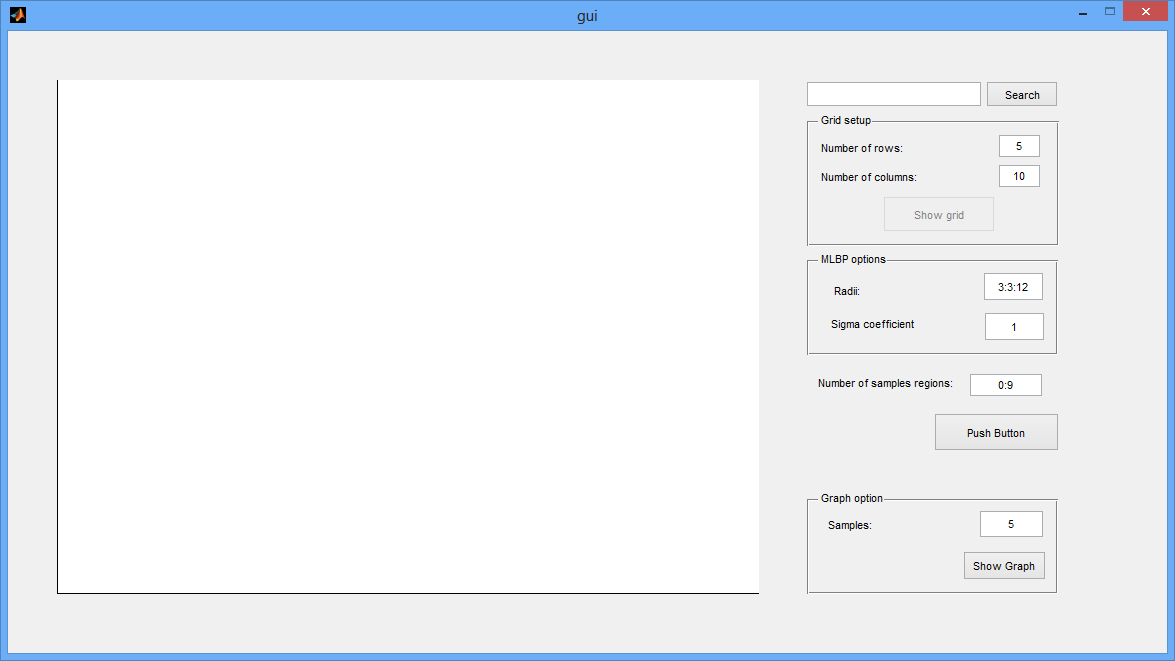
\includegraphics[width=.95\textwidth]{img/gui}
\caption{ GUI }
\label{fig:GUI}
\end{center}
\end{figure}

\subsection{Analisi dell'immagine}
- codice figo di lbp matrice
- mlbp += lbp + smoothing;

\subsubsection{Segmentazione}
- segmentazione bovina in regioni

\begin{figure}[ht]
\begin{center}
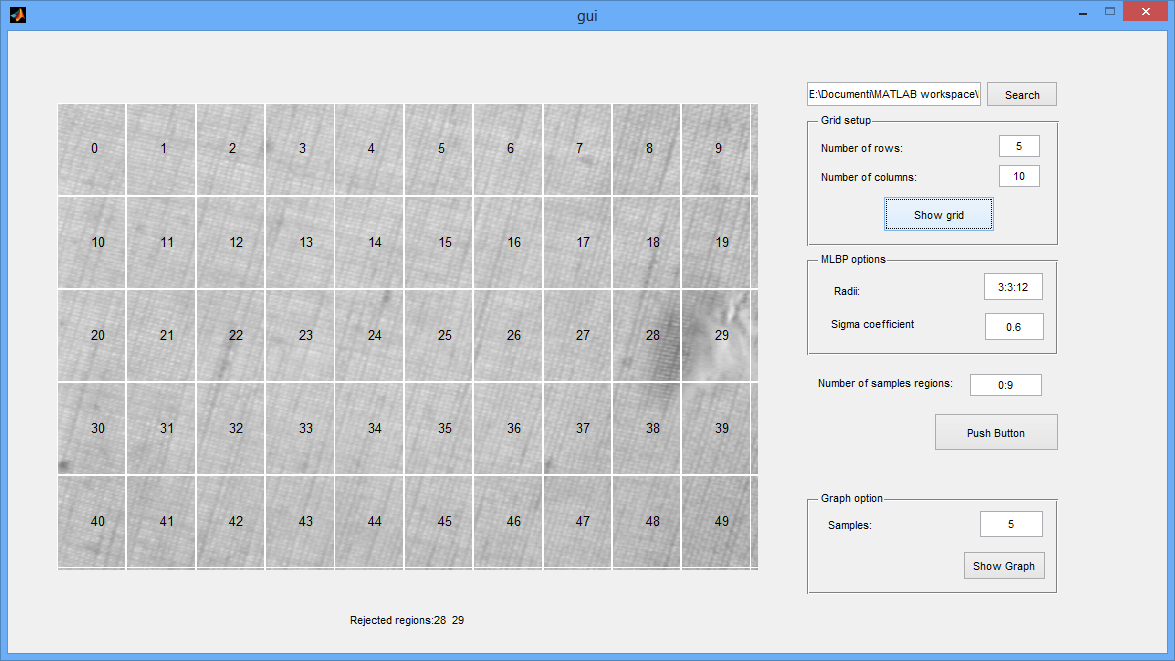
\includegraphics[width=.95\textwidth]{img/gui_pre_lbp}
\caption{ GUI pre LBP }
\label{fig:GUIpreLBP}
\end{center}
\end{figure}


- istogramma

\subsection{Misura di similarità}

Per misurare la similarità tra i descrittori di due regioni $I$ e $J$, possono essere utilizzati vari criteri. Abbiamo implementato le seguenti misure di similarità $Sim(I, J)$:

\begin{itemize}

\item Chi-square criterion:
\begin{equation}
Sim(I, J) = -  \sum_{i} \frac{ (f_{I}(i) - f_{J}(i) )^2}{f_{I}(i) + f_{J}(i)}
\end{equation}

\item Histogram intersection:
\begin{equation}
Sim(I, J) = \sum_{i} \mbox{min}(f_{I}(i),f_{J}(i))
\end{equation}

\item Log-likelihood ratio (Kullack-Leibler 
divergence):
\begin{equation}
Sim(I, J) = - \sum_{i} f_{I}(i)log(f_{J}(i)
\end{equation}

\item Normalize Correlation:
\begin{equation}
Sim(I, J) = \frac{f_{I}f_{J}'}{||f_{I}|| ||f_{J}||}
\end{equation}

\item Normalize Cross-correlation:
\begin{equation}
Sim(I, J) = \frac{\sigma_{f_{I}f_{J}}}{\sigma_{f_{I}}\sigma_{f_{J}}}
\end{equation}





j = regione
r = raggio
P = num neighbor
\begin{equation}
h_{P,r,j}(i) = \sum_{x',y' \in M_j} B(LBP_{P,r}(x', y')) = i, i \in  [0, L-1 ], r \in [1, R], j \in [0, J-1]
\end{equation}

\begin{equation}
B(v) = 	\begin{cases} 1, & \mbox{v = true} \\ 0, & \mbox{altrimenti} \end{cases}
\end{equation}

\begin{equation}
f_{j} = [h_{P, 1, j}, h_{P, 2, j}, \cdots, h_{P, R, j}]
\end{equation}

\end{itemize}


\subsection{Testing}
- regioni di training
- soglia di accettabilità 

\subsection{Risultati}
- risultati

\begin{figure}[ht]
\begin{center}
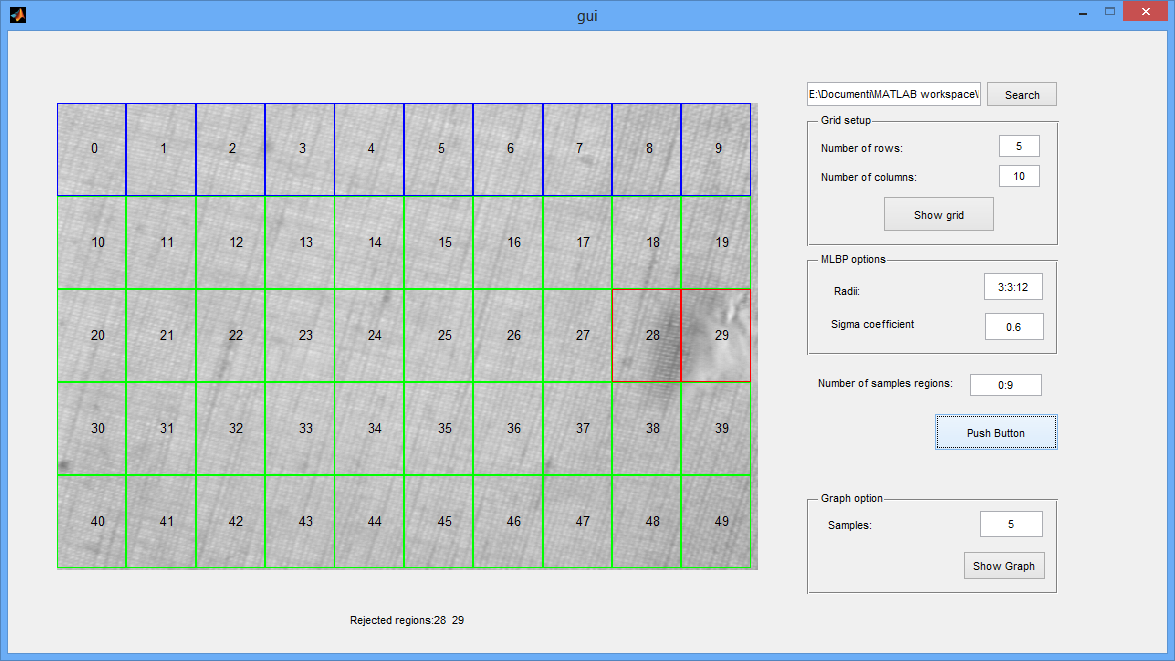
\includegraphics[width=.95\textwidth]{img/gui_post_lbp}
\caption{ GUI post LBP }
\label{fig:GUIpostLBP}
\end{center}
\end{figure}





\begin{figure}[ht]
\begin{center}
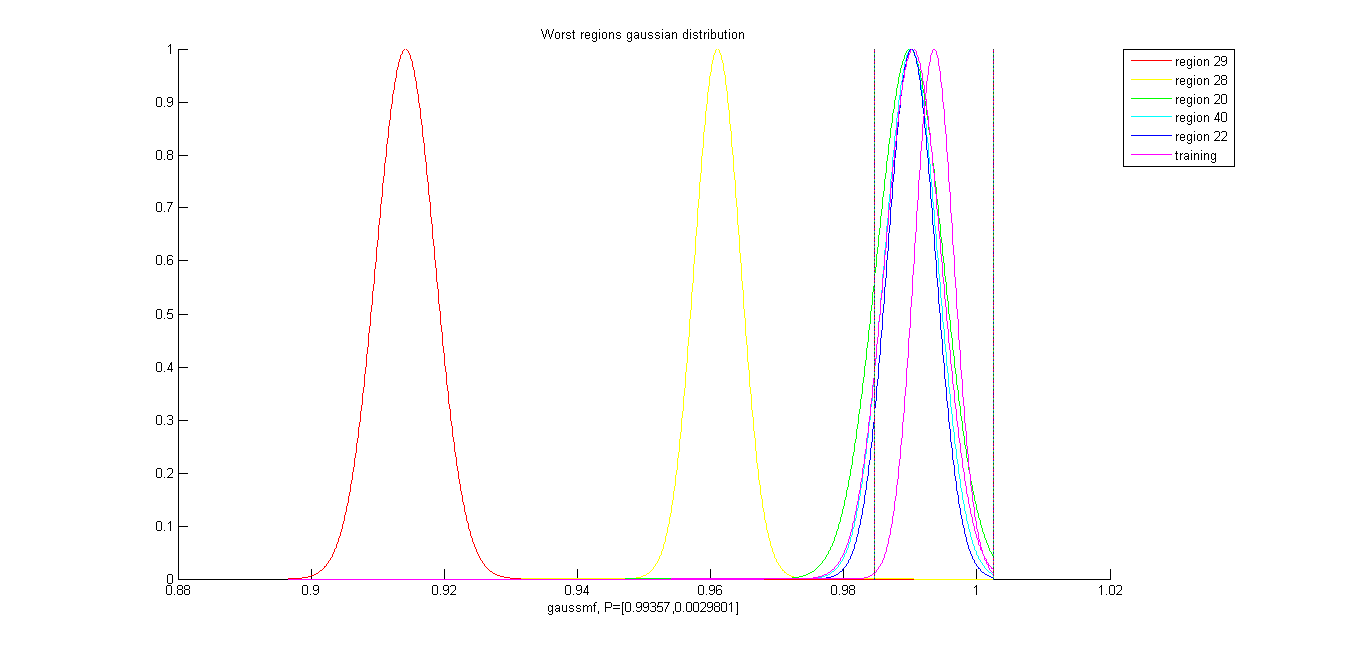
\includegraphics[width=.95\textwidth]{img/worst_graph}
\caption{ Caso peggiore }
\label{fig:worstGraph}
\end{center}
\end{figure}

\begin{figure}[ht]
\begin{center}
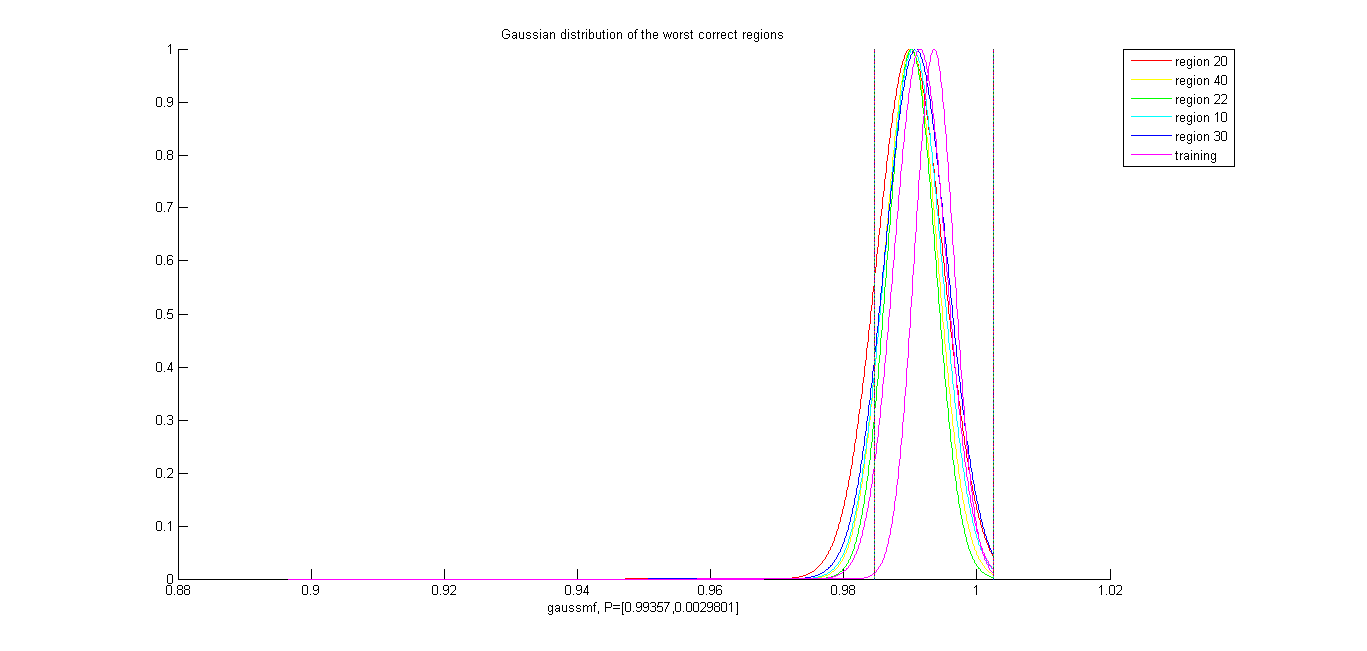
\includegraphics[width=.95\textwidth]{img/worst_best_graph}
\caption{ I peggiori tra i migliori }
\label{fig:worstBestGraph}
\end{center}
\end{figure}
